\section{Stacking-Probleme}
\label{sec:stacking_problems}

Stacking-Probleme treten in der Praxis zum Beispiel im Umfeld von Lagerhallen und Container-Terminals auf.
Ankommende \textit{Items}, häufig Container, müssen sogenannten \textit{Stacks} zugeordnet werden, sodass bestimmte Nebenbedingungen respektiert werden.
Diese Nebenbedingungen sorgen zum Beispiel dafür, dass nicht jedes \textit{Item} auf jedem anderen \textit{Item} platziert werden
darf. Es wird dabei angenommen, dass die im Folgenden als \textit{Storage-Area} bezeichnete Lagerfläche in festen
\textit{Stacks} organisiert ist, die eine limitierte gemeinsame Höhe besitzen, die im Folgenden als \textit{Stack}-Kapazität bezeichnet wird.\newline
Es kann in der Regel nur auf das oberste \textit{Item} eines \textit{Stacks} zugegriffen werden, d.h. der \textit{Item}-Zugriff erfolgt
nach dem \textquote{Last-In–First-Out}-Prinzip. Ein Zugriff auf \textit{Items} darunter erfordert eine \textit{Relocation}-Operation, die
zeit- und energieaufwendig ist.\newline

In dieser Arbeit wird nur der \textit{Loading}-Prozess betrachtet, währenddem keine \textit{Item}-Entnahme stattfindet.
Die \textit{Items} werden in die \textit{Storage-Area} geladen, die aus \textit{Stacks} mit einer festen Position besteht, d.h.
man kann die \textit{Stacks} nicht positionieren, sondern lediglich den \textit{Items} eine Position in einem \textit{Stack} zuweisen.\newline
Der \textit{Relocation}-Prozess wird typischerweise durch Kräne durchgeführt, die den \textit{Stacks} eine Maximalhöhe auferlegen.

Neben der Tatsache, dass nicht jedes \textit{Item} auf jedem anderen \textit{Item} platziert werden darf, gilt auch, dass es \textit{Items} gibt, die auf bestimmte Positionen beschränkt sind, weil sie zum Beispiel eine Energiequelle benötigen.
Abbildung \ref{fig:storage_area} zeigt den Aufbau der \textit{Storage-Area} bestehend aus $m$ fixierten
\textit{Stacks}, die jeweils $b$ \textit{Level} enthalten. Jedes \textit{Level} innerhalb eines \textit{Stacks} entspricht dabei einer Position, der ein \textit{Item} zugeordnet werden kann.

\begin{figure}[H]
\centering
\resizebox{0.5\textwidth}{!}{
\begin{tabular}{|c|c|c|c|c|c|}
\cline{1-5}
$\boldsymbol{S_1}$ & $\boldsymbol{S_2}$ & $\boldsymbol{S_3}$ & ... & $\boldsymbol{S_m}$\\ \cline{1-5}
\end{tabular}}
\caption*{\textsc{von oben betrachtet}}
\end{figure}
\begin{figure}[H]
\centering
\resizebox{0.5\textwidth}{!}{
\begin{tabular}{c|c|c|c|c|c|}
\cline{2-6}
$\boldsymbol{L_b}$ & $pos_{1, b}$ & $pos_{2, b}$ & $pos_{3, b}$ & ... & $pos_{m, b}$ \\ \cline{2-6}
... & ... & ... & ... & ... & ...\\ \cline{2-6}
$\boldsymbol{L_2}$ & $pos_{1, 2}$ & $pos_{2, 2}$ & $pos_{3, 2}$ & ... & $pos_{m, 2}$\\ \cline{2-6}
$\boldsymbol{L_1}$ & $pos_{1, 1}$ & $pos_{2, 1}$ & $pos_{3, 1}$ & ... & $pos_{m, 1}$\\ \cline{2-6}
\multicolumn{1}{c}{} & \multicolumn{1}{c}{$\boldsymbol{S_1}$} & \multicolumn{1}{c}{$\boldsymbol{S_2}$}
& \multicolumn{1}{c}{$\boldsymbol{S_3}$} & \multicolumn{1}{c}{...} & \multicolumn{1}{c}{$\boldsymbol{S_m}$} \\
\end{tabular}}
\caption*{\textsc{von der Seite betrachtet}}

\caption{\textsc{Aufbau der \textit{Storage-Area}}}
\label{fig:storage_area}
\end{figure}

Das Ziel von Stacking-Problemen ist es, jedes ankommende \textit{Item} einer zulässigen Position in einem
\textit{Stack} zuzuordnen, sodass eine gegebene Zielfunktion optimiert wird. Es gibt eine ganze Reihe praktisch relevanter Zielfunktionen,
in dieser Arbeit geht es um die Minimieren der Transportkosten, die bei der Verladung der \textit{Items} von ihrer Originalposition zur zugewiesenen Stackposition entstehen.

%%%%%%%%%%%%%%%%%%%%%%%%%%%%%%%%%%%%%%%%%%%%%%%%%%%%%%%%%%%%%%%%%%%%%%%%%%%%%%%%%%%%%%%%%%%%%%%%%%%%
\pagebreak
%%%%%%%%%%%%%%%%%%%%%%%%%%%%%%%%%%%%%%%%%%%%%%%%%%%%%%%%%%%%%%%%%%%%%%%%%%%%%%%%%%%%%%%%%%%%%%%%%%%%

\section{Formale Definition}
\label{sec:formal_definition}

Die \textit{Storage-Area} besteht aus \textit{Stacks}, die in einer Reihe angeordnet sind (vgl. Abb. \ref{fig:storage_area}). Die x-Koordinate spezifiziert jeweils den \textit{Stack} und die y-Koordinate den \textit{Level} innerhalb des jeweiligen \textit{Stacks}. Es handelt sich also um eine Reihe von $m$ \textit{Stacks} mit jeweils $b$ Positionen pro \textit{Stack}. Abb. \ref{fig:parameters} zeigt eine Liste der
Parameter, die im weiteren Verlauf der Arbeit immer wieder verwendet werden, um Stacking-Probleme zu definieren.
\begin{figure}[H]
\centering
\resizebox{0.5\textwidth}{!}{
\begin{tabular}{ | l | l |}
    \hline
    \textbf{Parameter} & \textbf{Semantik} \\ \hline
    $n$ & Anzahl der Items \\ \hline
    $m$ & Anzahl der Stacks \\ \hline
    $b$ & Stack Kapazität \\ \hline
    $I$ & Menge der Items $ I := \{1, 2, ..., n\}$ \\ \hline
\end{tabular}}
\caption{\textsc{Zur Definition verwendete Parameter}}
\label{fig:parameters}
\end{figure}
In der Regel gilt $m < n$, d.h. es müssen \textit{Items} gestapelt werden.
Außerdem muss die Annahme $n \leq bm$ gelten, denn sonst ist die Instanz des Problems unzulässig,
weil es mehr \textit{Items} als Positionen gibt.\newline
Für jedes \textit{Item} $i \in I$ ist dessen Originalposition $O_i$ in x- und y-Koordinaten gegeben.

\textit{Items}, die in einem \textit{Stack} platziert werden, sind durch ein Tupel $(i_k, ..., i_1)$ definiert, wobei
$i_\lambda$ das \textit{Item} auf \textit{Level} $\lambda$ beschreibt. $\lambda = 1$ beschreibt den \textit{Ground-Level}.
Instanzen können Stacking-Restriktionen $s_{ij}$ enthalten, die angeben, ob ein \textit{Item} $i$ direkt auf einem \textit{Item} $j$ platziert
werden darf. Dies ist der Fall, wenn $s_{ij} = 1$ gilt.
Ein Tupel ist zulässig, wenn $k \leq b$ und $s_{i_{\lambda + 1}, i_\lambda} = 1 \quad \forall \quad \lambda = 1, ..., k - 1$.
D.h. ein Tupel ist dann zulässig, wenn die \textit{Stack}-Kapazität eingehalten wird und alle \textit{Items}, die aufeinander gestapelt sind,
nicht den Stacking-Restriktionen widersprechen, die in Kapitel \ref{stacking_restrictions} erläutert werden.

\textbf{Formulierung des Problems}\newline
Gegeben sei eine Menge $I = \{1, ..., n\}$ von \textit{Items} und eine Menge $Q = \{1, ..., m\}$ von \textit{Stacks} mit einer \textit{Stack}-Kapazität von $b$. Außerdem seien \textit{Stacking Constraints} $s_{ij}$ und \textit{Placement Constraints} $t_{iq}$ gegeben.
Das Ziel ist nun, jedes \textit{Item} $i \in I$ genau einem \textit{Stack} $q \in Q$ zuzuweisen, wobei die \textit{Stacking Constraints} $s_{ij}$,
die Placement Constraints $t_{iq}$ und die Stack-Kapazität $b$ respektiert werden und gegebenenfalls eine Zielfunktion optimiert wird.

%%%%%%%%%%%%%%%%%%%%%%%%%%%%%%%%%%%%%%%%%%%%%%%%%%%%%%%%%%%%%%%%%%%%%%%%%%%%%%%%%%%%%%%%%%%%%%%%%%%%
\pagebreak
%%%%%%%%%%%%%%%%%%%%%%%%%%%%%%%%%%%%%%%%%%%%%%%%%%%%%%%%%%%%%%%%%%%%%%%%%%%%%%%%%%%%%%%%%%%%%%%%%%%%

\section{Das Zulässigkeitsproblem}
\label{sec:decision_problem}

Die simpelste Variante des Storage Loading Problems ist ein Zulässigkeitsproblem, welches die Frage stellt, ob sämtliche Items der Storage Area zugewiesen werden können, sodass alle Nebenbedingungen respektiert werden.
Diese Nebenbedingungen beziehen sich z.B. auf die Stack Kapazität, die Stacking Constraints, ein Gewichtslimit pro Stack oder auch
Restriktionen bezüglich der Position.\newline
Sollte dies möglich sein, so ist häufig das Ziel, jedes Item einer zulässigen Position zuzuweisen.
Diese Position zeichnet sich durch einen Stack-Index und einen Level innerhalb des Stacks aus.
Dabei kann z.B. eine der in Abb. \ref{fig:objective_functions} dargestellten Zielfunktionen optimiert werden, was jedoch bereits über
das Zulässigkeitsproblem hinausgeht.

%%%%%%%%%%%%%%%%%%%%%%%%%%%%%%%%%%%%%%%%%%%%%%%%%%%%%%%%%%%%%%%%%%%%%%%%%%%%%%%%%%%%%%%%%%%%%%%%%%%%
\pagebreak
%%%%%%%%%%%%%%%%%%%%%%%%%%%%%%%%%%%%%%%%%%%%%%%%%%%%%%%%%%%%%%%%%%%%%%%%%%%%%%%%%%%%%%%%%%%%%%%%%%%%

\section{Transportkosten}
\label{sec:transport_costs}
Die Transportkosten beziehen sich auf die Kosten, die bei der Verladung der \textit{Items} in die \textit{Storage-Area} entstehen
und sind praktisch zum Beispiel durch Kranbetriebskosten, Wartezeiten oder auch Arbeitszeiten motiviert.\newline
Jeder Stack $q$ besitzt eine fixierte Position $F_q$ in der Storage-Area. Außerdem besitzt jedes Item $i$ eine gegebene
Originalposition $O_i$ auf dem Fahrzeug, mit dem es geliefert wird. Die Kosten ergeben sich aus der Manhattan-Distanz zwischen
Item- und zugewiesener Stack-Position, da diese der Kranbewegung entspricht. In Abb. \ref{fig:costs} ist dieser Sachverhalt visualisiert.
\begin{figure}[H]
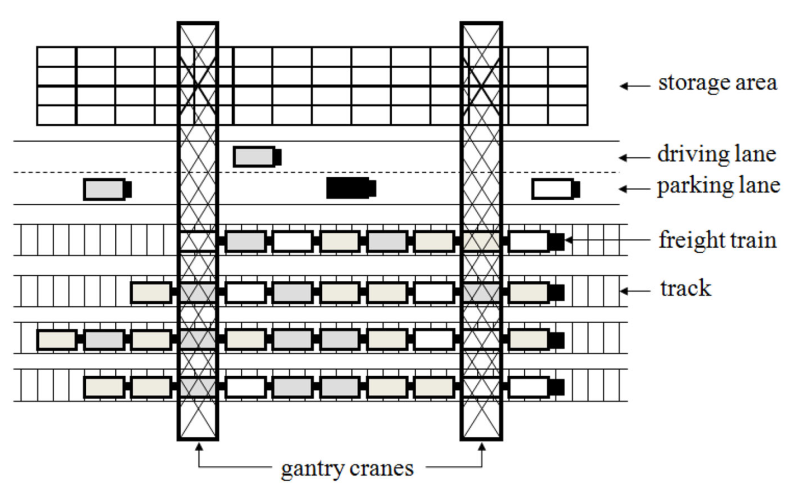
\includegraphics[width=\textwidth]{img/costs.png}
\caption{Beispielszenario}
\label{fig:costs}
\end{figure}
Die Transportkosten werden in einer Matrix $C = (c_{iq})_{n \times m}$ kodiert, \newline wobei $c_{iq} \coloneqq d_{man}(O_i, F_q)$.

%%%%%%%%%%%%%%%%%%%%%%%%%%%%%%%%%%%%%%%%%%%%%%%%%%%%%%%%%%%%%%%%%%%%%%%%%%%%%%%%%%%%%%%%%%%%%%%%%%%%
\pagebreak
%%%%%%%%%%%%%%%%%%%%%%%%%%%%%%%%%%%%%%%%%%%%%%%%%%%%%%%%%%%%%%%%%%%%%%%%%%%%%%%%%%%%%%%%%%%%%%%%%%%%

\section{Nebenbedingungen}
\label{sec:constraints}

\subsection{Stacking Restriktionen}
\label{sec:stacking_restrictions}

Es gibt in der Praxis vielfältige Gründe dafür, dass nicht jedes \textit{Item} auf jedes andere \textit{Item} gestapelt werden darf.
Aus diesen resultieren bestimmte Restriktionen, die z.B. wie folgt lauten:
\begin{itemize}
  \item schwerere \textit{Items} dürfen nicht auf leichteren \textit{Items} platziert werden
  \item größere \textit{Items} dürfen nicht auf kleineren \textit{Items} platziert werden
  \item \textit{Items} bestimmter Materialien oder Zielorte dürfen nicht aufeinander gestapelt werden
\end{itemize}

All jene Restriktionen, die im Folgenden stets als \textit{Stacking Constraints} bezeichnet werden, werden in einer Binärmatrix $S = (s_{ij})_{n \times n}$ kodiert, wobei:
\[
    s_{ij} =
\begin{cases}
    1, & \text{wenn $i$ direkt auf $j$ gestapelt werden darf }\\
    0, & \text{sonst}
\end{cases}
\]
Diese Matrix lässt sich, wie in Abb. \ref{fig:matrix_to_graph} beispielhaft dargestellt,
als gerichteter Graph mit $n$ Knoten für alle $i \in I$ und Kanten $i \rightarrow j$ für alle $s_{ij} = 1$ repräsentieren.
\begin{figure}[H]
  \begin{subfigure}[b]{0.5\textwidth}
  \centering
    $S =$
    $\left(
    \begin{array}{rrrr}
    0 & 1 & 1 & 0 \\
    1 & 0 & 1 & 0 \\
    1 & 0 & 0 & 0 \\
    1 & 1 & 1 & 0 \\
    \end{array} \right) $
    \caption{\textsc{Constraint Matrix}}
    \label{fig:constraint_matrix}
  \end{subfigure}
  \hfill
  \begin{subfigure}[b]{0.5\textwidth}
  \centering
    \begin{tikzpicture}[->, scale=0.50, transform shape, node distance=2.5cm]
    \node[state] (A) {1};
    \node[state] (B) [right of=A] {2};
    \node[state] (C) [below of=A] {3};
    \node[state] (D) [right of=C] {4};

    \path (A) edge node {} (B)
          (A) edge node {} (C)

          (B) edge [bend right] node {} (A)
          (B) edge [bend left=10] node {} (C)

          (C) edge [bend left] node {} (A)

          (D) edge [bend left=10] node {} (A)
          (D) edge node {} (B)
          (D) edge node {} (C);
  \end{tikzpicture}
    \caption{\textsc{Resultierender Graph}}
    \label{fig:resulting_graph}
  \end{subfigure}
  \caption{\textsc{Stacking Constraints interpretiert als Matrix bzw. Graph.}}
  \label{fig:matrix_to_graph}
\end{figure}
\textit{Stacking Constraints} können transitiv sein. Ist dies der Fall, so gilt folgendes:\newline
Wenn \textit{Item} $i$ auf \textit{Item} $j$ und \textit{Item} $j$ auf \textit{Item} $h$ gestapelt werden darf,
so darf auch \textit{Item} $i$ auf \textit{Item} $h$ gestapelt werden.\newline
Restriktionen bezüglich des Gewichts und der Länge haben die besondere Eigenschaft, dass alle Items vergleichbar sind, d.h. für alle $i \neq j  \quad \text{gilt} \quad s_{ij} = 1 \quad \text{oder} \quad s_{ji} = 1$, was bedeutet, dass diese Restriktionen eine totale Ordnung auf allen \textit{Items} definieren.

%%%%%%%%%%%%%%%%%%%%%%%%%%%%%%%%%%%%%%%%%%%%%%%%%%%%%%%%%%%%%%%%%%%%%%%%%%%%%%%%%%%%%%%%%%%%%%%%%%%%
\pagebreak
%%%%%%%%%%%%%%%%%%%%%%%%%%%%%%%%%%%%%%%%%%%%%%%%%%%%%%%%%%%%%%%%%%%%%%%%%%%%%%%%%%%%%%%%%%%%%%%%%%%%

\subsection{Placement Restriktionen}
\label{sec:placement_restrictions}

Die im Folgenden als \textit{Placement Constraints} bezeichneten Einschränkungen bezüglich der Position eines Items resultieren z.B.
aus der Länge oder dem Gewicht der Items und den Eigenschaften der Stacks oder auch durch spezielle Anforderungen der Items wie
Kühlcontainer, die eine Energiequelle benötigen. Tendenziell sind dabei mehr Item-Stack-Zuweisungen erlaubt als verboten.
Diese Placement-Constraints werden nun allerdings nicht direkt implementiert, sondern indirekt über hohe Kostenwerte.\newline

Zunächst werden die Placement-Constraints in einer Binärmatrix $\boldsymbol{T} = (\boldsymbol{t_{iq}})_{n \times m}$ kodiert, wobei:\newline
$
    \boldsymbol{t_{iq}} =
\begin{cases}
    1, & \text{wenn Item $\boldsymbol{i}$ in Stack $\boldsymbol{q}$ platziert werden darf }\\
    0, & \text{sonst}
\end{cases}
$
\\[20pt]

Diese Matrix wird jedoch nicht direkt verwendet, um die Restriktionen zu implementieren. Stattdessen wird
die Transportkosten-Matrix $C$ nun wie folgt erweitert.

Für die Transportkosten-Matrix $\boldsymbol{C} = (\boldsymbol{c_{iq}})_{n \times m}$ gilt:\newline
$
    \boldsymbol{c_{iq}} =
\begin{cases}
    d_{man}(\boldsymbol{O_i}, \boldsymbol{F_q}), & \text{wenn $\boldsymbol{t_{iq}} = 1$}\\
    \infty, & \text{sonst}
\end{cases}
$

%%%%%%%%%%%%%%%%%%%%%%%%%%%%%%%%%%%%%%%%%%%%%%%%%%%%%%%%%%%%%%%%%%%%%%%%%%%%%%%%%%%%%%%%%%%%%%%%%%%%
\pagebreak
%%%%%%%%%%%%%%%%%%%%%%%%%%%%%%%%%%%%%%%%%%%%%%%%%%%%%%%%%%%%%%%%%%%%%%%%%%%%%%%%%%%%%%%%%%%%%%%%%%%%

\section{Problemstellungen}
\label{sec:problem_settings}

\subsection{Komplexität}
\label{sec:complexity}

In diesem Kapitel werden konkret die Problemstellungen eingeführt, die im Folgenden heuristisch gelöst werden.
Es werden die Stack-Kapazitäten $b=2, b=3 $ und $ b=4$ betrachtet, die besonders in Szenarien aus der Praxis, in denen
Container gestapelt werden, von Interesse sind.

Wie \cite{Bruns2015} zeigte, handelt es sich bei dem Zulässigkeitsproblem mit $b=3$ und gegebenen $s_{ij}$ um
ein NP-vollständiges Problem. Erst kürzlich wurde außerdem gezeigt, dass auch $b=2$ mit gegebenen $s_{ij}$ und $t_{iq}$
NP-vollständig ist. Somit sind auch die entsprechenden Stacking-Probleme, die zusätzlich die Transportkosten minimieren, NP-vollständig.

\subsection{Instanzgrößen}
\label{sec:instance_sizes}

Die betrachteten Testinstanzen werden in drei Kategorien unterteilt:
\begin{itemize}
  \item klein (\textbf{s}) ($\leq 100$ Items)
  \item mittel (\textbf{m}) ($\approx 300$ Items)
  \item groß (\textbf{l}) ($\approx 500$ Items)\newline
\end{itemize}
Dies scheint auch in der Literatur der Rahmen zu sein, in dem sich solche Stacking-Probleme typischerweise bewegen.

\subsection{Ziel}
\label{sec:objective}

Sämtliche Items sollen möglichst günstig eingelagert werden, d.h. die Zielfunktion entspricht der Minimierung der Transportkosten.
Dabei haben Zulässigkeit und geringe Laufzeit allerdings Priorität.


%%%%%%%%%%%%%%%%%%%%%%%%%%%%%%%%%%%%%%%%%%%%%%%%%%%%%%%%%%%%%%%%%%%%%%%%%%%%%%%%%%%%%%%%%%%%%%%%%%%%
\pagebreak
%%%%%%%%%%%%%%%%%%%%%%%%%%%%%%%%%%%%%%%%%%%%%%%%%%%%%%%%%%%%%%%%%%%%%%%%%%%%%%%%%%%%%%%%%%%%%%%%%%%%

\section{Testdaten-Generierung}
\label{sec:test_data}

In diesem Kapitel geht es um die durchaus interessante Frage danach, wie realistische Test-Instanzen aussehen können.
Zunächst einmal werden pro Konfiguration 20 Instanzen verwendet um eine Vergleichbarkeit zu ermöglichen.
Die Anzahl der Items $n$ sowie die Stack-Kapazität $b$ wird stets spezifiziert und in der Berechnung der Anzahl
der zur Verfügung stehenden Stacks $m$ verwendet: $m$ = $\ceil{n / b}$ + $20 \%$.\newline
Bei einer Stackanzahl von $m$ = $\ceil{n / b}$ gäbe es überhaupt keinen Spielraum bei der Itemplatzierung. Ein Spielraum von $20 \%$
ist durchaus gering und könnte in weiteren Betrachtungen erhöht werden.

\textbf{Stacking-Constraint-Generierung}\newline

Es wurden zwei Varianten der Stacking-Constraint-Generierung implementiert, die im Folgenden erläutert werden.

\textbf{Variante 1}\newline
Die Stacking-Constraint Matrix $S$ wird anhand einer definierten Wahrscheinlichkeit mit $1$- bzw. $0$-Einträgen gefüllt.
Anschließend werden die 1-Einträge, die aus Transitivität folgen, ergänzt.

\textbf{Variante 2}\newline
Für alle $n$ Items wird eine zufällige Länge und Breite generiert. Item $i$ kann auf Item $j$ platziert werden,
wenn für dessen Länge $l_i$ und Breite $w_i$ gilt $l_i \leq l_j$ und $w_i \leq w_j$.
Items $i, j$ sind in beide Richtungen stackbar, wenn $l_i = l_j$ und $w_i = w_j$.

Variante 2 scheint realitätsnäher zu sein und wird deshalb zunächst bevorzugt. Aufgrund der Tatsache, dass Variante 2 jedoch stets
zu einer 1-Quote von ca. 25\% führt und diese mit Variante 1 sehr gut konfigurierbar ist, wird Variante 1 jedoch noch nicht vollständig verworfen.
(TODO: Grund ergänzen...)

Bei den Placement-Constraints sind in den betrachteten Tests 70\% der Item-Stack-Zuweisungen erlaubt.
Zur Transportkostenberechnung wird wie in Abschnitt \ref{sec:transport_costs} erläutert, die Manhattan-Metrik verwendet. Dazu sind
entsprechend die Item- und Stackpositionen als x- und y-Koordinaten gegeben. Auch die entsprechenden Längen und Breiten sowie die Distanz zwischen Storage-Area und den Fahrzeug-Lanes ist jeweils gegeben.

%%%%%%%%%%%%%%%%%%%%%%%%%%%%%%%%%%%%%%%%%%%%%%%%%%%%%%%%%%%%%%%%%%%%%%%%%%%%%%%%%%%%%%%%%%%%%%%%%%%%
\pagebreak
%%%%%%%%%%%%%%%%%%%%%%%%%%%%%%%%%%%%%%%%%%%%%%%%%%%%%%%%%%%%%%%%%%%%%%%%%%%%%%%%%%%%%%%%%%%%%%%%%%%%

\section{MIP-Formulierungen}
\label{sec:mip_formulations}

In diesem Abschnitt werden die MIP-Formulierungen eingeführt, die zum experimentellen Vergleich genutzt werden.
Es geht darum, mit den MIP-Formulierungen die optimalen Zielfunktionswerte der Instanzen zu ermitteln, um dann
zu ermitteln, wie weit die Heuristiken davon abweichen. Des Weiteren geht es auch um einen Vergleich der MIP-Formulierungen
untereinander.

\subsection{Bin-Packing-Formulierung}
\label{sec:bin_packing_formulation}

\begin{gather}
\boldsymbol{min} \quad \sum_{i \in I} \sum_{q \in Q} c_{iq} x_{iq} \\
\thinspace\thinspace \boldsymbol{s.t.} \thinspace\quad\thinspace\thinspace\thinspace\quad\thinspace \quad \sum_{q \in Q} x_{iq} = 1 \quad\quad\quad\quad\quad\quad\quad \forall i \in I \quad\quad\quad\quad\thinspace\thinspace \\
\quad \sum_{i \in I} x_{iq} \leq b \quad\quad\quad\quad\quad\quad\quad \forall q \in Q \\
\thinspace\thinspace\quad\quad x_{iq} + x_{jq} \leq 1 \quad\quad\thinspace\thinspace\quad\quad\quad\quad \forall \{i, j\} \notin A \\
\thinspace\thinspace\quad\quad\quad x_{iq} \in \{0, 1\} \thinspace\thinspace\thinspace\thinspace\thinspace\thinspace\quad\quad\quad\quad\quad\quad \forall i \in I, q \in Q \thinspace
\end{gather}

\subsection{3-Index-Formulierung}
\label{sec:three_idx_formulation}

\begin{gather}
\boldsymbol{min} \quad \sum_{i \in I} \sum_{q \in Q} \sum_{l \in L} c_{iq} x_{iql} \\
\boldsymbol{s.t.} \quad \sum_{q \in Q} \sum_{l \in L} x_{iql} = 1 \quad\thinspace\thinspace\quad\quad\quad\quad \forall i \in I \thinspace\thinspace\quad\quad\quad\quad\quad\quad\quad\quad\thinspace\thinspace \\
\sum_{i \in I} x_{iql} \leq 1 \thinspace\quad\quad\quad\quad\quad\quad\quad \forall q \in Q, l \in L \thinspace\thinspace\thinspace\thinspace\quad\quad\quad\thinspace \\
\sum_{j \in I | i \rightarrow j} x_{jq(l-1)} - x_{iql} \geq 0 \thinspace\quad\quad \forall i \in I, q \in Q, l \in L \textbackslash \{1\} \\
\quad\quad x_{iql} \in \{0, 1\} \quad\quad\quad\quad\quad\quad\quad \forall i \in I, q \in Q, l \in L \quad\thinspace\thinspace\thinspace\thinspace\thinspace
\end{gather}


%%%%%%%%%%%%%%%%%%%%%%%%%%%%%%%%%%%%%%%%%%%%%%%%%%%%%%%%%%%%%%%%%%%%%%%%%%%%%%%%%%%%%%%%%%%%%%%%%%%%
\pagebreak
%%%%%%%%%%%%%%%%%%%%%%%%%%%%%%%%%%%%%%%%%%%%%%%%%%%%%%%%%%%%%%%%%%%%%%%%%%%%%%%%%%%%%%%%%%%%%%%%%%%%

\section{Konstruktive Heuristiken}
\label{sec:constructive_heuristics}

In diesem Abschnitt werden die entwickelten konstruktiven Heuristiken vorgestellt.
Zunächst werden drei wichtige Konzepte vorgestellt, in \ref{sec:digression_mcm} das Maximum-Cardinality-Matching,
in \ref{sec:digression_mwpm} das Minimum-Weight-Perfect-Matching und in \ref{sec:digression_bipartite_graph} ein
bipartiter Graph.

\subsection{Exkurs: Maximum-Cardinality-Matching (MCM)}
\label{sec:digression_mcm}

Gegeben sei ein ungerichteter Graph $G = (V, E)$. Eine Menge $M \subseteq E$ heißt Matching,
wenn keine zwei Kanten aus $M$ einen Knoten gemeinsam haben. Falls $M$ als Menge eine maximale Kardinalität unter
allen Matchings von $G$ hat, wird dies als Maximum-Cardinality-Matching bezeichnet. \cite{WikiMatching}
Es kann mehrere unterschiedliche MCMs in einem Graphen geben.
In Abb. \ref{fig:mcm_examples} werden beispielhaft zwei MCMs dargestellt.
\begin{figure}[H]
  \begin{subfigure}[b]{0.4\textwidth}
  \centering
    \begin{tikzpicture}[scale=0.45, transform shape, node distance=2cm]
    \node[state] (A) {};
    \node[state] (B) [above right of=A] {};
    \node[state] (C) [below left of=A] {};
    \node[state] (D) [below right of=C] {};
    \node[state] (F) [below right of=B] {};
    \node[state] (E) [below of=F] {};

    \path (A) edge [red] node {} (B)
          (A) edge node {} (C)
          (A) edge node {} (D)
          (A) edge node {} (E)
          (A) edge node {} (F)
          (C) edge [red] node {} (D);
  \end{tikzpicture}
  \caption{\textsc{$|MCM| = 2$}}
  \label{fig:mcm1}
  \end{subfigure}
  \hfill
  \begin{subfigure}[b]{0.4\textwidth}
  \centering
    \begin{tikzpicture}[scale=0.45, transform shape, node distance=2cm]
    \node[state] (A) {};
    \node[state] (B) [right of=A] {};
    \node[state] (C) [right of=B] {};
    \node[state] (D) [below left of=A] {};
    \node[state] (E) [below right of=D] {};
    \node[state] (F) [right of=E] {};

    \path (A) edge node {} (B)
          (B) edge [red] node {} (C)
          (B) edge node {} (F)
          (A) edge node {} (E)
          (E) edge [red] node {} (F)
          (A) edge [red] node {} (D)
          (D) edge node {} (E);
  \end{tikzpicture}
    \caption{\textsc{$|MCM| = 3$}}
    \label{fig:mcm_2}
  \end{subfigure}
  \caption{\textsc{Zwei Beispiele für MCMs (dargestellt in rot).}}
  \label{fig:mcm_examples}
\end{figure}

\subsection{Exkurs: Minimum-Weight-Perfect-Matching}
\label{sec:digression_mwpm}

Zunächst einmal ist es wichtig, zu erwähnen, dass ein Perfect-Matching nur für Graphen mit einer geraden Anzahl an Knoten möglich ist.
Ein Perfect-Matching ist ein Matching, welches sämtliche Knoten des Graphen matcht.
D.h. jeder Knoten des Graphen ist inzident zu genau einer Kante des Matchings (vgl. Abb. \ref{fig:perfect_matching}).
Ein Minimum-Weight-Perfect-Matching ist nun ein günstigstes Perfect-Matching basierend auf den Kantenkosten.
\begin{figure}[H]
\centering
\begin{tikzpicture}[-, scale=0.40, transform shape, node distance=3cm]
    \node[state] (A) {};
    \node[state] (B) [above right of=A] {};
    \node[state] (C) [below right of=A] {};
    \node[state] (D) [right of=B] {};
    \node[state] (E) [right of=D] {};
    \node[state] (F) [right of=C] {};

    \path (A) edge [red] node {} (B)
          (A) edge node {} (C)
          (B) edge node {} (D)
          (B) edge node {} (C)
          (D) edge [red] node {} (E)
          (D) edge node {} (F)
          (C) edge [red] node {} (F);
\end{tikzpicture}
\caption{\textsc{Beispiel für ein Perfect-Matching (rot).}}
\label{fig:perfect_matching}
\end{figure}

\subsection{Exkurs: Bipartiter Graph}
\label{sec:digression_bipartite_graph}

Ein Graph $G = (V, E)$ heißt bipartit (vgl. Abb. \ref{fig:bipartite_graph}), wenn die Knotenmenge in zwei disjunkte Teilmengen zerfällt
$(V = S \cup T$ mit $S \cap T = \emptyset$), sodass jede Kante einen Knoten aus $S$ mit einem Knoten aus $T$ verbindet. \cite{HochschuleDarmstadt}\newline
Es lassen sich folgende Äquivalenzen festhalten:
\begin{itemize}
  \item $G$ bipartit $\iff$ $G$ 2-färbbar
  \item $G$ bipartit $\iff$ keine Kreise ungerader Länge in $G$
\end{itemize}

\begin{figure}[H]
\centering
\begin{tikzpicture}[scale=0.50, transform shape, node distance=3cm]
  \node[state] [green] (A) {};
  \node[state] [red] (B) [above right of=A] {};
  \node[state] [green] (C) [below right of=B] {};
  \node[state] [red] (D) [below of=B] {};
  \node[state] [red] (E) [below of=A] {};
  \node[state] [green] (F) [right of=E] {};

  \path (A) edge node {} (B)
        (B) edge node {} (C)
        (C) edge node {} (D)
        (A) edge node {} (D)
        (A) edge node {} (E)
        (E) edge node {} (F)
        (D) edge node {} (F);

\end{tikzpicture}
\caption{\textsc{Bipartiter Graph.}}
\label{fig:bipartite_graph}
\end{figure}

\subsection{Konstruktive Heuristik ($b = 2$)}
\label{sec:two_cap_heuristic}

\begin{itemize}
  \item Stacking-Constraint-Graph generieren
  \item \textsc{\textbf{MCM}} berechnen, Kanten als Item-Paare interpretieren
  \item Bipartiten Graph generieren:
  \begin{enumerate}
    \item Items (Item-Paare, Unmatched-Items)
    \item Stacks
  \end{enumerate}
  \item \textsc{\textbf{MWPM}} berechnen, Kanten als Stackzuweisungen interpretieren
  \item Ggf. Reihenfolge der Items innerhalb der Stacks anpassen
\end{itemize}

\textbf{Beispiel}
$\boldsymbol{I} := \{0, 1, 2, 3, 4, 5, 6\} \quad\quad\quad \boldsymbol{b} := 2 \quad\quad\quad \boldsymbol{m} := 4$
\begin{figure}[H]
    \centering
    \begin{tikzpicture}[scale=0.8, transform shape, node distance=3cm]
        \node[state] (G) [thick] {$\boldsymbol{6}$};
        \node[state] (B) [thick, above left of=G] {$\boldsymbol{1}$};
        \node[state] (C) [thick, above right of=G] {$\boldsymbol{2}$};
        \node[state] (E) [thick, below right of=G] {$\boldsymbol{4}$};
        \node[state] (F) [thick, below left of=G] {$\boldsymbol{5}$};
        \node[state] (A) [thick, below left of=B] {$\boldsymbol{0}$};
        \node[state] (D) [thick, below right of=C] {$\boldsymbol{3}$};

        \path (B) edge [thick] node {} (C)
              (B) edge [thick] node {} (F)
              (B) edge [thick] node {} (G)
              (C) edge [thick, bend right = 75, distance=5cm] node {} (F)
              (C) edge [thick] node {} (E)
              (C) edge [thick] node {} (D)
              (C) edge [thick] node {} (G)
              (F) edge [thick] node {} (G)
              (F) edge [thick] node {} (E)
              (E) edge [thick] node {} (G);
    \end{tikzpicture}
    \caption*{\textsc{Stacking-Constraint-Graph}}
\end{figure}


\begin{figure}[H]
  \centering
  \begin{tikzpicture}[scale=0.7, transform shape, node distance=3cm]
        \node[state] (G) [thick] {$\boldsymbol{\textcolor{mygreen}{6}}$};
        \node[state] (B) [thick, above left of=G] {$\boldsymbol{\textcolor{mygreen}{1}}$};
        \node[state] (C) [thick, above right of=G] {$\boldsymbol{\textcolor{mygreen}{2}}$};
        \node[state] (E) [thick, below right of=G] {$\boldsymbol{\textcolor{mygreen}{4}}$};
        \node[state] (F) [thick, below left of=G] {$\boldsymbol{\textcolor{mygreen}{5}}$};
        \node[state] (A) [thick, below left of=B] {$\boldsymbol{\textcolor{red}{0}}$};
        \node[state] (D) [thick, below right of=C] {$\boldsymbol{\textcolor{mygreen}{3}}$};

        \path (B) edge [thick] node {} (C)
              (B) edge [thick] node {} (F)
              (B) edge [thick, mygreen] node {} (G)
              (C) edge [thick, bend right = 75, distance=5cm] node {} (F)
              (C) edge [thick] node {} (E)
              (C) edge [thick, mygreen] node {} (D)
              (C) edge [thick] node {} (G)
              (F) edge [thick] node {} (G)
              (F) edge [thick, mygreen] node {} (E)
              (E) edge [thick] node {} (G);
    \end{tikzpicture}
  \caption*{\textsc{MCM (Item $0$ unmatched)}}
\end{figure}


\begin{figure}[H]
\centering
\begin{tikzpicture}[scale=0.7, transform shape, node distance=3cm]
        \node[state] (A) [thick] {\textcolor{mygreen}{$\boldsymbol{1, 6}$}};
        \node[state] (B) [thick, right of=A] {\textcolor{mygreen}{$\boldsymbol{2, 3}$}};
        \node[state] (C) [thick, right of=B] {\textcolor{mygreen}{$\boldsymbol{4, 5}$}};
        \node[state] (D) [thick, right of=C] {\textcolor{red}{$\boldsymbol{0}$}};
        \path ;
  \end{tikzpicture}
  \caption*{\textsc{Kanten bilden Item-Paare}}
\end{figure}

\begin{figure}[H]
\begin{subfigure}[b]{0.45\textwidth}
\centering
\begin{tikzpicture}[scale=0.7, transform shape, node distance=1.5cm]
        \node[state] (A) [thick] {$\boldsymbol{1, 6}$};
        \node[state] (B) [thick, below of=A] {$\boldsymbol{2, 3}$};
        \node[state] (C) [thick, below of=B] {$\boldsymbol{4, 5}$};
        \node[state] (D) [thick, below of=C] {$\boldsymbol{0}$};

        \node[state] (F) [thick, right = 4cm of A] {$\boldsymbol{S_1}$};
        \node[state] (G) [thick, right = 4cm of B] {$\boldsymbol{S_2}$};
        \node[state] (H) [thick, right = 4cm of C] {$\boldsymbol{S_3}$};
        \node[state] (I) [thick, right = 4cm of D] {$\boldsymbol{S_4}$};

        \path
          % from (1,6) to all stacks
          (A) edge [thick] node {} (F)
          (A) edge [thick] node {} (G)
          (A) edge [thick] node {} (H)
          (A) edge [thick] node {} (I)

          % from (2,3) to all stacks
          (B) edge [thick] node {} (F)
          (B) edge [thick] node {} (G)
          (B) edge [thick] node {} (H)
          (B) edge [thick] node {} (I)

          % from (4,5) to all stacks
          (C) edge [thick] node {} (F)
          (C) edge [thick] node {} (G)
          (C) edge [thick] node {} (H)
          (C) edge [thick] node {} (I)

          % from 0 to all stacks
          (D) edge [thick] node {} (F)
          (D) edge [thick] node {} (G)
          (D) edge [thick] node {} (H)
          (D) edge [thick] node {} (I);
  \end{tikzpicture}
  \caption*{\textsc{vollständig bipartit}}
\end{subfigure}
\hfill
\begin{subfigure}[b]{0.45\textwidth}
\centering
\begin{tikzpicture}[scale=0.7, transform shape, node distance=1.5cm]
        \node[state] (A) [thick] {$\boldsymbol{1, 6}$};
        \node[state] (B) [thick, below of=A] {$\boldsymbol{2, 3}$};
        \node[state] (C) [thick, below of=B] {$\boldsymbol{4, 5}$};
        \node[state] (D) [thick, below of=C] {$\boldsymbol{0}$};

        \node[state] (F) [thick, right = 4cm of A] {$\boldsymbol{S_1}$};
        \node[state] (G) [thick, right = 4cm of B] {$\boldsymbol{S_2}$};
        \node[state] (H) [thick, right = 4cm of C] {$\boldsymbol{S_3}$};
        \node[state] (I) [thick, right = 4cm of D] {$\boldsymbol{S_4}$};

        \path
          (A) edge [thick] node {} (I)
          (B) edge [thick] node {} (H)
          (C) edge [thick] node {} (G)
          (D) edge [thick] node {} (F);
  \end{tikzpicture}
  \caption*{\textsc{MWPM}}
\end{subfigure}
\end{figure}

\begin{figure}[H]
  \centering
  \resizebox{0.4\textwidth}{!}{
    \begin{tabular}{c|c|c|c|c|}
    \cline{2-5}
    $\boldsymbol{L_2}$ & $$ & $5$ & $3$ & $6$ \\ \cline{2-5}
    $\boldsymbol{L_1}$ & $0$ & $4$ & $2$ & $1$ \\ \cline{2-5}
    \multicolumn{1}{c}{} & \multicolumn{1}{c}{$\boldsymbol{S_1}$} & \multicolumn{1}{c}{$\boldsymbol{S_2}$}
    & \multicolumn{1}{c}{$\boldsymbol{S_3}$} & \multicolumn{1}{c}{$\boldsymbol{S_4}$} \\
    \end{tabular}}
    \caption*{\textsc{Zulässige Zuweisungen (ggf. Item-Reihenfolge korrigieren)}}
\end{figure}

\pagebreak

\subsection{Vergleich der $b = 2$ Solver (s)}
\label{sec:solver_comp_b=2_s}

\begin{figure}[H]
\centering
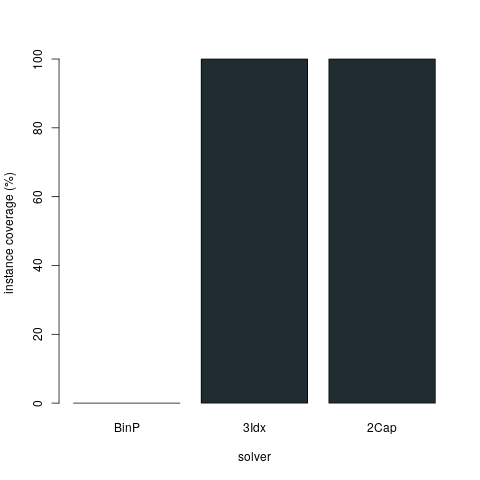
\includegraphics[width=0.3\textwidth]{img/solver_instance_coverage_b=2_s_1s.png}
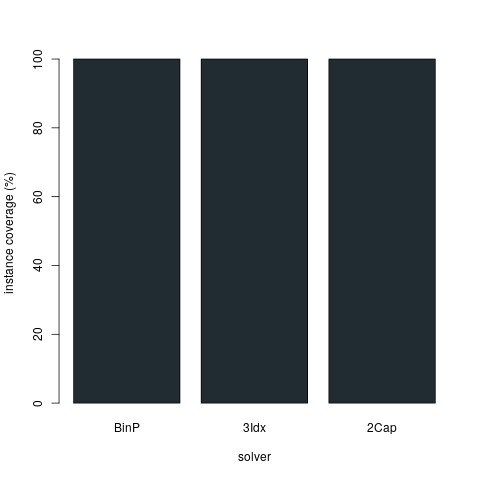
\includegraphics[width=0.3\textwidth]{img/solver_instance_coverage_b=2_s_3s.png}
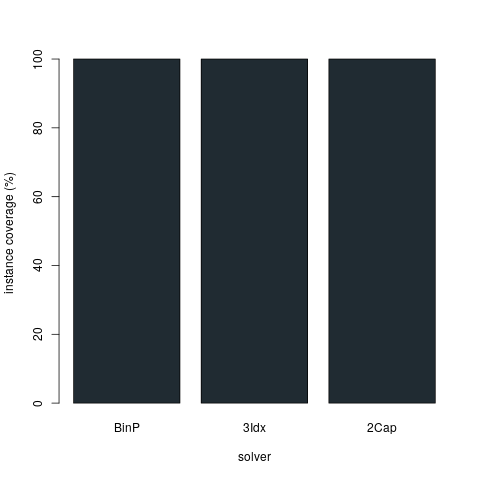
\includegraphics[width=0.3\textwidth]{img/solver_instance_coverage_b=2_s_5s.png}
\caption*{\textsc{Zeitlimit} $1s$ $\quad\quad\quad\thinspace\thinspace\thinspace\thinspace\thinspace$ \textsc{Zeitlimit} $3s$
$\thinspace\thinspace\thinspace\thinspace\thinspace\quad\quad\quad$ \textsc{Zeitlimit} $5s$}
% \end{figure}
% \begin{figure}[H]
\begin{subfigure}[b]{0.3\textwidth}
\centering
\resizebox{\textwidth}{!}{
\begin{tabular}{ | l | l | l |}
    \hline
     & \textbf{BinP} & \textbf{3Idx} \\ \hline
    \textbf{Optimal} & $ \textcolor{red}{0 \%}$ & $ \textcolor{mygreen}{35 \%}$ \\ \hline
    \textbf{Laufzeit} & $\textcolor{red}{---}$ & \O $\thinspace \textcolor{mygreen}{0.9 s}$ \\ \hline
    \textbf{Abweichung} & $\textcolor{red}{---}$ & \O $\thinspace \textcolor{mygreen}{2.0 \%}$ \\ \hline
\end{tabular}}
\end{subfigure}
% $\quad\quad\quad\quad$
\begin{subfigure}[b]{0.3\textwidth}
\centering
\resizebox{\textwidth}{!}{
\begin{tabular}{ | l | l | l |}
    \hline
     & \textbf{BinP} & \textbf{3Idx} \\ \hline
    \textbf{Optimal} & $ \textcolor{red}{10 \%}$ & $ \textcolor{mygreen}{100 \%}$ \\ \hline
    \textbf{Laufzeit} & \O $\thinspace \textcolor{red}{3.0 s}$ & \O $\thinspace \textcolor{mygreen}{1.1 s}$ \\ \hline
    \textbf{Abweichung} & \O $\thinspace \textcolor{red}{4.7 \%}$ & \O $\thinspace \textcolor{mygreen}{0.0 \%}$ \\ \hline
\end{tabular}}
\end{subfigure}
% \end{figure}
% \begin{figure}[H]
\begin{subfigure}[b]{0.3\textwidth}
\centering
\resizebox{\textwidth}{!}{
\begin{tabular}{ | l | l | l |}
    \hline
     & \textbf{BinP} & \textbf{3Idx} \\ \hline
    \textbf{Optimal} & $ \textcolor{red}{90 \%}$ & $ \textcolor{mygreen}{100 \%}$ \\ \hline
    \textbf{Laufzeit} & \O $\thinspace \textcolor{red}{3.9 s}$ & \O $\thinspace \textcolor{mygreen}{1.1 s}$ \\ \hline
    \textbf{Abweichung} & \O $\thinspace \textcolor{red}{0.4 \%}$ & \O $\thinspace \textcolor{mygreen}{0.0 \%}$ \\ \hline
\end{tabular}}
\end{subfigure}
\end{figure}
\centering
\textbf{2Cap-Heuristik}\linebreak
\centering
Abweichung vom Optimum: \O $\thinspace \boldsymbol{2.0 \%}$\linebreak
\centering
Laufzeit: \O $\thinspace \boldsymbol{0.02 s}$

\subsection{Vergleich der $b = 2$ Solver (m)}
\label{sec:solver_comp_b=2_m}

\begin{figure}[H]
\centering
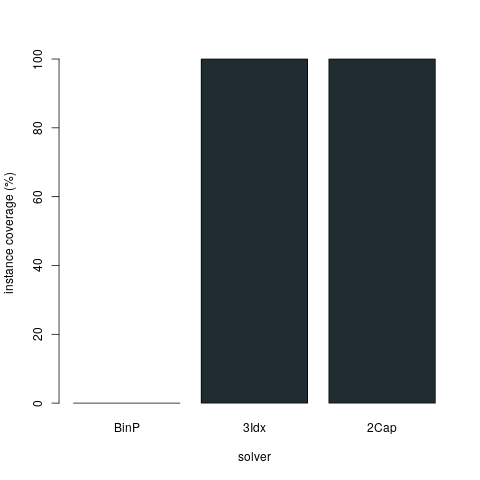
\includegraphics[width=0.3\textwidth]{img/solver_instance_coverage_b=2_m_60s.png}
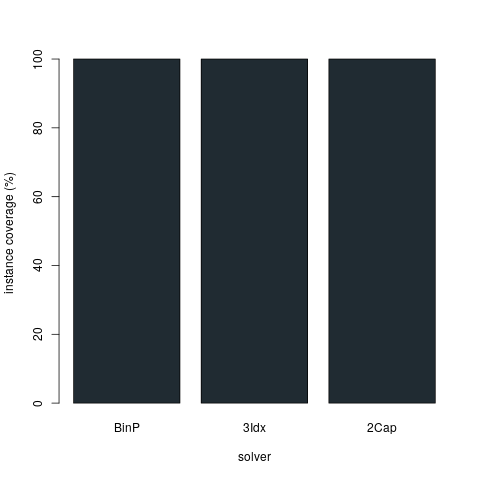
\includegraphics[width=0.3\textwidth]{img/solver_instance_coverage_b=2_m_600s.png}
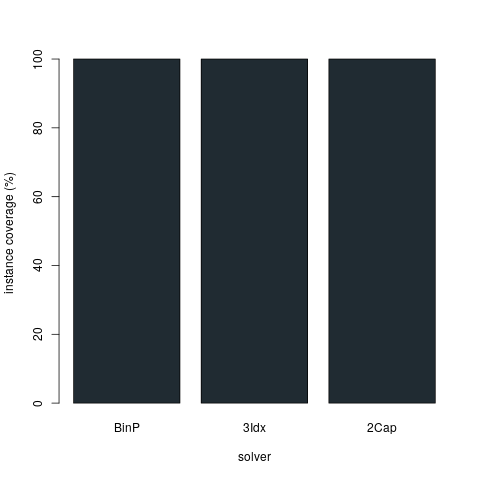
\includegraphics[width=0.3\textwidth]{img/solver_instance_coverage_b=2_m_1200s.png}
\caption*{\textsc{Zeitlimit} $1min$ $\quad\quad\quad$ \textsc{Zeitlimit} $10min$ $\quad\quad\quad$ \textsc{Zeitlimit} $20min$}
% \end{figure}
% \begin{figure}[H]
% $\quad\quad\quad\quad$
\begin{subfigure}[b]{0.3\textwidth}
\centering
\resizebox{\textwidth}{!}{
\begin{tabular}{ | l | l | l |}
    \hline
     & \textbf{BinP} & \textbf{3Idx} \\ \hline
    \textbf{Optimal} & $ \textcolor{red}{0 \%}$ & $ \textcolor{mygreen}{50 \%}$ \\ \hline
    \textbf{Laufzeit} & $\textcolor{red}{----}$ & \O $\thinspace \textcolor{mygreen}{55.4 s}$ \\ \hline
    \textbf{Abweichung} & $\textcolor{red}{----}$ & \O $\thinspace \textcolor{mygreen}{0.8 \%}$ \\ \hline
\end{tabular}}
\end{subfigure}
\begin{subfigure}[b]{0.3\textwidth}
\centering
\resizebox{\textwidth}{!}{
\begin{tabular}{ | l | l | l |}
    \hline
     & \textbf{BinP} & \textbf{3Idx} \\ \hline
    \textbf{Optimal} & $ \textcolor{red}{10 \%}$ & $ \textcolor{mygreen}{100 \%}$ \\ \hline
    \textbf{Laufzeit} & \O $\thinspace \textcolor{red}{581.6 s}$ & \O $\thinspace \textcolor{mygreen}{73.7 s}$ \\ \hline
    \textbf{Abweichung} & \O $\thinspace \textcolor{red}{0.6 \%}$ & \O $\thinspace \textcolor{mygreen}{0.0 \%}$ \\ \hline
\end{tabular}}
\end{subfigure}
% \end{figure}
% \begin{figure}[H]
\begin{subfigure}[b]{0.3\textwidth}
\centering
\resizebox{\textwidth}{!}{
\begin{tabular}{ | l | l | l |}
    \hline
     & \textbf{BinP} & \textbf{3Idx} \\ \hline
    \textbf{Optimal} & $ 100 \%$ & $ 100 \%$ \\ \hline
    \textbf{Laufzeit} & \O $\thinspace 869.6 s$ & \O $\thinspace \textcolor{mygreen}{107.8 s}$ \\ \hline
    \textbf{Abweichung} & \O $\thinspace 0.0 \%$ & \O $\thinspace 0.0 \%$ \\ \hline
\end{tabular}}
\end{subfigure}
\end{figure}
\centering
\textbf{2Cap-Heuristik}\linebreak
\centering
Abweichung vom Optimum: \O $\thinspace \boldsymbol{0.8 \%}$\linebreak
\centering
Laufzeit: \O $\thinspace \boldsymbol{0.1 s}$

\pagebreak

\subsection{Vergleich der $b = 2$ Solver (l)}
\label{sec:solver_comp_b=2_l}

\begin{figure}[H]
\centering
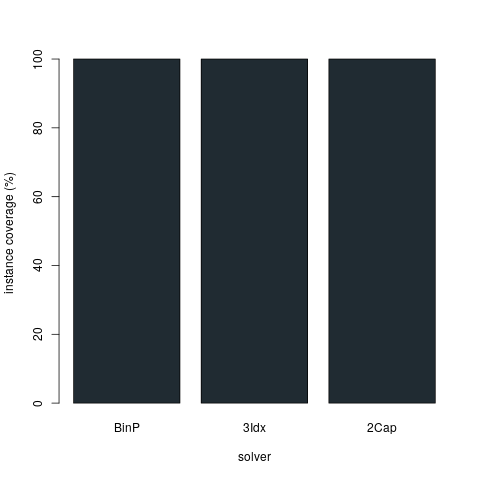
\includegraphics[width=0.3\textwidth]{img/solver_instance_coverage_b=2_l_900s.png}
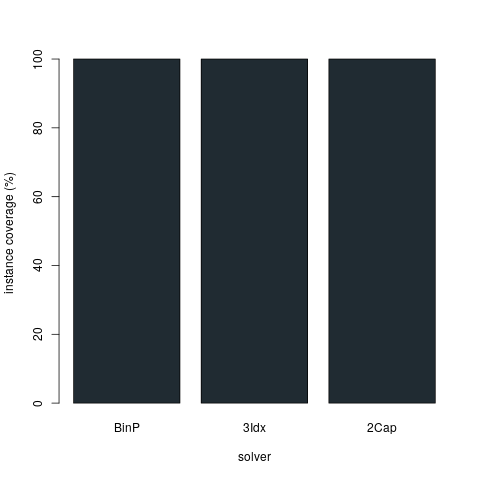
\includegraphics[width=0.3\textwidth]{img/solver_instance_coverage_b=2_l_1800s.png}
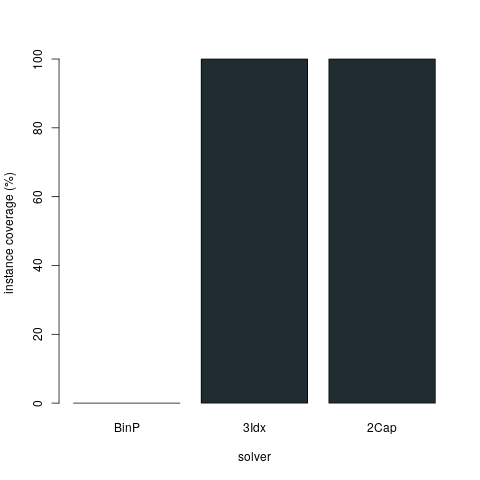
\includegraphics[width=0.3\textwidth]{img/solver_instance_coverage_b=2_l_2700s.png}
\caption*{\textsc{Zeitlimit} $15min$ $\quad\quad\quad$ \textsc{Zeitlimit} $30min$ $\quad\quad\quad$ \textsc{Zeitlimit} $45min$}
% \end{figure}
% \begin{figure}[H]
\begin{subfigure}[b]{0.3\textwidth}
\centering
\resizebox{\textwidth}{!}{
\begin{tabular}{ | l | l | l |}
    \hline
     & \textbf{BinP} & \textbf{3Idx} \\ \hline
    \textbf{Optimal} & $ \textcolor{red}{0 \%}$ & $ \textcolor{mygreen}{70 \%}$ \\ \hline
    \textbf{Laufzeit} & \textcolor{red}{$---$} & \O $\thinspace \textcolor{mygreen}{728.0 s}$ \\ \hline
    \textbf{Abweichung} & \textcolor{red}{$---$} & \O $\thinspace \textcolor{mygreen}{0.53 \%}$ \\ \hline
\end{tabular}}
\end{subfigure}
\begin{subfigure}[b]{0.3\textwidth}
\centering
\resizebox{\textwidth}{!}{
\begin{tabular}{ | l | l | l |}
    \hline
     & \textbf{BinP} & \textbf{3Idx} \\ \hline
    \textbf{Optimal} & $ \textcolor{red}{0 \%}$ & $ \textcolor{mygreen}{85 \%}$ \\ \hline
    \textbf{Laufzeit} & \textcolor{red}{$---$} & \O $\thinspace \textcolor{mygreen}{977.2 s}$ \\ \hline
    \textbf{Abweichung} & \textcolor{red}{$---$} & \O $\thinspace \textcolor{mygreen}{0.0 \%}$ \\ \hline
\end{tabular}}
\end{subfigure}
% $\quad\quad\quad\quad$
\begin{subfigure}[b]{0.3\textwidth}
\centering
\resizebox{\textwidth}{!}{
\begin{tabular}{ | l | l | l |}
    \hline
     & \textbf{BinP} & \textbf{3Idx} \\ \hline
    \textbf{Optimal} & $ \textcolor{red}{0 \%}$ & $ \textcolor{mygreen}{100 \%}$ \\ \hline
    \textbf{Laufzeit} & \textcolor{red}{$---$} & \O $\thinspace \textcolor{mygreen}{1185.9  s}$ \\ \hline
    \textbf{Abweichung} & \textcolor{red}{$---$} & \O $\thinspace \textcolor{mygreen}{0.0 \%}$ \\ \hline
\end{tabular}}
\end{subfigure}
% \end{figure}
% \begin{figure}[H]
\end{figure}
\centering
\textbf{2Cap-Heuristik}\linebreak
\centering
Abweichung vom Optimum: \O $\thinspace \boldsymbol{0.6 \%}$\linebreak
\centering
Laufzeit: \O $\thinspace \boldsymbol{0.7 s}$

\subsection{Konstruktive Heuristik ($b = 3$)}
\label{sec:three_cap_heuristic}

\begin{itemize}
  \item Item-Paare bilden (\textsc{\textbf{MCM}(items)})
  \item Item-Tripel bilden (\textsc{\textbf{MCM}(pairs, unmatchedItems)})
  \item Verbleibende Item-Paare zu Tripeln mergen
  \item Item-Paare bilden (\textsc{\textbf{MCM}(remainingItems)})
  \item Verbleibende Items als \textquote{unmatched} betrachten
  \item Bipartiten Graph generieren:
  \begin{enumerate}
    \item Items (Item-Tripel, Item-Paare, Unmatched-Items)
    \item Stacks
  \end{enumerate}
  \item \textsc{\textbf{MWPM}} berechnen, Kanten als Stackzuweisungen interpretieren
  \item Ggf. Reihenfolge der Items innerhalb der Stacks anpassen
\end{itemize}

\pagebreak

\textbf{Beispiel}
$\boldsymbol{I} := \{0, 1, 2, 3, 4, 5, 6, 7, 8, 9\} \quad\quad\quad \boldsymbol{b} := 3 \quad\quad\quad \boldsymbol{m} := 4$
\begin{figure}[H]
\centering
\begin{tikzpicture}[scale=0.65, transform shape, node distance=2cm]
        \node[state] (A) [thick] {$\boldsymbol{\textcolor{mygreen}{0, 2}}$};
        \node[state] (B) [thick, right of=A] {$\boldsymbol{\textcolor{mygreen}{1, 9}}$};
        \node[state] (C) [thick, right of=B] {$\boldsymbol{\textcolor{mygreen}{3, 4}}$};
        \node[state] (D) [thick, right of=C] {$\boldsymbol{\textcolor{mygreen}{5, 6}}$};
        \node[state] (E) [thick, right of=D] {$\boldsymbol{\textcolor{red}{7}}$};
        \node[state] (F) [thick, right of=E] {$\boldsymbol{\textcolor{red}{8}}$};
        \path;
  \end{tikzpicture}
  \caption*{\textsc{Item-Paare und Unmatched-Items}}
% \end{figure}
% \begin{figure}[H]
\centering
\begin{tikzpicture}[scale=0.65, transform shape, node distance=2cm]
        \node[state] (A) [thick] {$\boldsymbol{\textcolor{red}{0, 2}}$};
        \node[state] (B) [thick, right of=A] {$\boldsymbol{\textcolor{red}{1, 9}}$};
        \node[state] (C) [thick, right of=B] {$\boldsymbol{\textcolor{mygreen}{3, 4}}$};
        \node[state] (D) [thick, right of =C] {$\boldsymbol{\textcolor{red}{5, 6}}$};
        \node[state] (E) [thick, right of=D] {$\boldsymbol{\textcolor{mygreen}{7}}$};
        \node[state] (F) [thick, right of=E] {$\boldsymbol{\textcolor{red}{8}}$};
        \path
          (E) edge [thick, mygreen, bend right] node {} (C)
          (E) edge [thick] node {} (D);
  \end{tikzpicture}
  \caption*{\textsc{MCM aus Item-Paaren und Unmatched-Items}}
% \end{figure}
% \begin{figure}[H]
\centering
\begin{tikzpicture}[scale=0.65, transform shape, node distance=2cm]
        \node[state] (A) [thick] {$\boldsymbol{3, 4, 7}$};
        \node[state] (B) [thick, right of=A] {$\boldsymbol{0, 2}$};
        \node[state] (C) [thick, right of=B] {$\boldsymbol{1, 9}$};
        \node[state] (D) [thick, right of=C] {$\boldsymbol{5, 6}$};
        \node[state] (E) [thick, right of=D] {$\boldsymbol{8}$};
        \path;
\end{tikzpicture}
\caption*{\textsc{Item-Tripel, Item-Paare und Unmatched-Items}}
\begin{subfigure}[b]{0.4\textwidth}
\centering
\begin{tikzpicture}[scale=0.65, transform shape, node distance=2cm]
        \node[state] (A) [thick] {$\boldsymbol{0, 2}$};
        \node[state] (B) [thick, right of=A] {$\boldsymbol{1, 9}$};
        \node[state] (C) [thick, right of=B] {$\boldsymbol{5, 6}$};
        \path;
  \end{tikzpicture}
  \caption*{\textsc{Item-Paare}}
\end{subfigure}
\hspace{10pt}
\begin{subfigure}[b]{0.4\textwidth}
\centering
\begin{tikzpicture}[scale=0.65, transform shape, node distance=2cm]
        \node[state] (A) [thick] {$\boldsymbol{0, 5, 6}$};
        \node[state] (B) [thick, right of=A] {$\boldsymbol{2, 1, 9}$};
        \path;
  \end{tikzpicture}
  \caption*{\textsc{Merge-Ergebnis}}
\end{subfigure}

\end{figure}

\begin{figure}[H]
% \begin{figure}[H]
\begin{subfigure}[b]{0.4\textwidth}
\centering
\begin{tikzpicture}[scale=0.65, transform shape, node distance=2cm]
        \node[state] (A) [thick] {$\boldsymbol{3, 4, 7}$};
        \node[state] (B) [thick, below of=A] {$\boldsymbol{0, 5, 6}$};
        \node[state] (C) [thick, below of=B] {$\boldsymbol{2, 1, 9}$};
        \node[state] (D) [thick, below of=C] {$\boldsymbol{8}$};

        \node[state] (E) [thick, right = 4cm of A] {$\boldsymbol{S_1}$};
        \node[state] (F) [thick, below of=E] {$\boldsymbol{S_2}$};
        \node[state] (G) [thick, below of=F] {$\boldsymbol{S_3}$};
        \node[state] (H) [thick, below of=G] {$\boldsymbol{S_4}$};

        \path
          (A) edge [thick] node {} (E)
          (A) edge [thick] node {} (F)
          (A) edge [thick] node {} (G)
          (A) edge [thick] node {} (H)

          (B) edge [thick] node {} (E)
          (B) edge [thick] node {} (F)
          (B) edge [thick] node {} (G)
          (B) edge [thick] node {} (H)

          (C) edge [thick] node {} (E)
          (C) edge [thick] node {} (F)
          (C) edge [thick] node {} (G)
          (C) edge [thick] node {} (H)

          (D) edge [thick] node {} (E)
          (D) edge [thick] node {} (F)
          (D) edge [thick] node {} (G)
          (D) edge [thick] node {} (H);
  \end{tikzpicture}
  \caption*{\textsc{Vollständig Bipartit}}
\end{subfigure}
\hfill
\begin{subfigure}[b]{0.4\textwidth}
\centering
\begin{tikzpicture}[scale=0.65, transform shape, node distance=2cm]
        \node[state] (A) [thick] {$\boldsymbol{3, 4, 7}$};
        \node[state] (B) [thick, below of=A] {$\boldsymbol{0, 5, 6}$};
        \node[state] (C) [thick, below of=B] {$\boldsymbol{2, 1, 9}$};
        \node[state] (D) [thick, below of=C] {$\boldsymbol{8}$};

        \node[state] (E) [thick, right = 4cm of A] {$\boldsymbol{S_1}$};
        \node[state] (F) [thick, below of=E] {$\boldsymbol{S_2}$};
        \node[state] (G) [thick, below of=F] {$\boldsymbol{S_3}$};
        \node[state] (H) [thick, below of=G] {$\boldsymbol{S_4}$};

        \path
          (A) edge [thick] node {} (H)
          (B) edge [thick] node {} (F)
          (C) edge [thick] node {} (G)
          (D) edge [thick] node {} (E);
  \end{tikzpicture}
  \caption*{\textsc{MWPM}}
\end{subfigure}
% \end{figure}
\newline\newline
% \begin{figure}[H]
  \centering
  \resizebox{0.35\textwidth}{!}{
    \begin{tabular}{c|c|c|c|c|}
    \cline{2-5}
    $\boldsymbol{L_3}$ & $$ & $6$ & $9$ & $7$ \\ \cline{2-5}
    $\boldsymbol{L_2}$ & $$ & $5$ & $1$ & $4$ \\ \cline{2-5}
    $\boldsymbol{L_1}$ & $8$ & $0$ & $2$ & $3$ \\ \cline{2-5}
    \multicolumn{1}{c}{} & \multicolumn{1}{c}{$\boldsymbol{S_1}$} & \multicolumn{1}{c}{$\boldsymbol{S_2}$}
    & \multicolumn{1}{c}{$\boldsymbol{S_3}$} & \multicolumn{1}{c}{$\boldsymbol{S_4}$} \\
    \end{tabular}}
    \caption*{\textsc{Zulässige Zuweisungen (ggf. Item-Reihenfolge korrigieren)}}
\end{figure}

\pagebreak

\subsection{Vergleich der $b = 3$ Solver (s)}
\label{sec:solver_comp_b=3_s}

\begin{figure}[H]
\centering
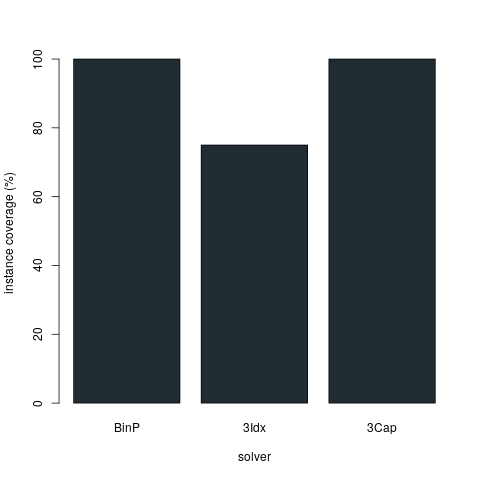
\includegraphics[width=0.3\textwidth]{img/solver_instance_coverage_b=3_s_3s.png}
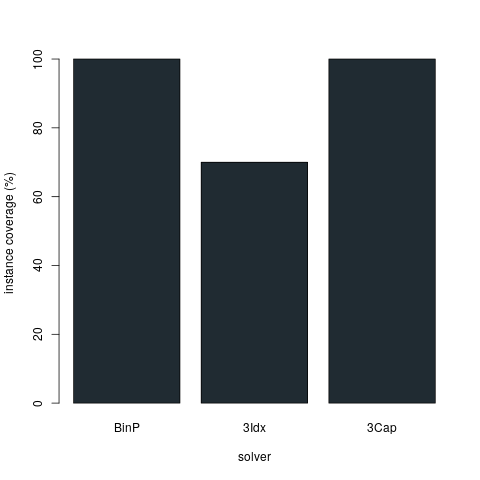
\includegraphics[width=0.3\textwidth]{img/solver_instance_coverage_b=3_s_5s.png}
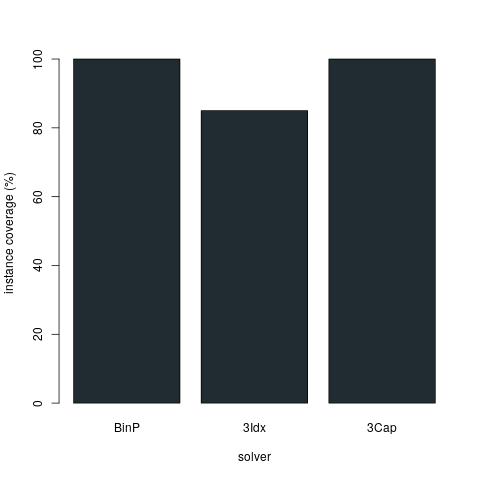
\includegraphics[width=0.3\textwidth]{img/solver_instance_coverage_b=3_s_10s.png}
\caption*{\textsc{Zeitlimit} $3s$ $\quad\quad\quad\quad$ \textsc{Zeitlimit} $5s$ $\quad\quad\quad\quad$ \textsc{Zeitlimit} $10s$}
% \end{figure}
% \begin{figure}[H]
% $\quad\quad\quad\quad$
\begin{subfigure}[b]{0.3\textwidth}
\centering
\resizebox{\textwidth}{!}{
\begin{tabular}{ | l | l | l |}
    \hline
     & \textbf{BinP} & \textbf{3Idx} \\ \hline
    \textbf{Optimal} & $\textcolor{mygreen}{40 \%}$ & $\textcolor{red}{5 \%}$ \\ \hline
    \textbf{Laufzeit} & \O $\thinspace 2.9 s$ & \O $\thinspace 2.9 s$ \\ \hline
    \textbf{Abweichung} & \O $\thinspace \textcolor{mygreen}{1.7 \%}$ & \O $\thinspace \textcolor{red}{7.8 \%}$ \\ \hline
\end{tabular}}
\end{subfigure}
% \end{figure}
% \begin{figure}[H]
\begin{subfigure}[b]{0.3\textwidth}
\centering
\resizebox{\textwidth}{!}{
\begin{tabular}{ | l | l | l |}
    \hline
     & \textbf{BinP} & \textbf{3Idx} \\ \hline
    \textbf{Optimal} & $\textcolor{mygreen}{100 \%}$ & $\textcolor{red}{50 \%}$ \\ \hline
    \textbf{Laufzeit} & \O $\thinspace \textcolor{mygreen}{3.1 s}$ & \O $\thinspace \textcolor{red}{4.0 s}$ \\ \hline
    \textbf{Abweichung} & \O $\thinspace \textcolor{mygreen}{0.0 \%}$ & \O $\thinspace \textcolor{red}{1.2 \%}$ \\ \hline
\end{tabular}}
\end{subfigure}
\begin{subfigure}[b]{0.3\textwidth}
\centering
\resizebox{\textwidth}{!}{
\begin{tabular}{ | l | l | l |}
    \hline
     & \textbf{BinP} & \textbf{3Idx} \\ \hline
    \textbf{Optimal} & $ \textcolor{mygreen}{100 \%}$ & $ \textcolor{red}{85 \%}$ \\ \hline
    \textbf{Laufzeit} & \O $\thinspace \textcolor{mygreen}{3.1 s}$ & \O $\thinspace \textcolor{red}{5.6 s}$ \\ \hline
    \textbf{Abweichung} & \O $\thinspace \textcolor{mygreen}{0.0 \%}$ & \O $\thinspace \textcolor{red}{0.5 \%}$ \\ \hline
\end{tabular}}
\end{subfigure}
\end{figure}
\centering
\textbf{3Cap-Heuristik}\linebreak
\centering
Abweichung vom Optimum: \O $\thinspace \boldsymbol{2.65 \%}$\linebreak
\centering
Laufzeit: \O $\thinspace \boldsymbol{0.01s}$

\subsection{Vergleich der $b = 3$ Solver (m)}
\label{sec:solver_comp_b=3_m}

\begin{figure}[H]
\centering
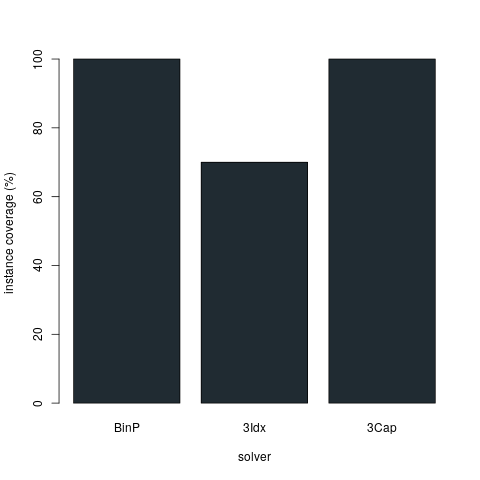
\includegraphics[width=0.3\textwidth]{img/solver_instance_coverage_b=3_m_600s.png}
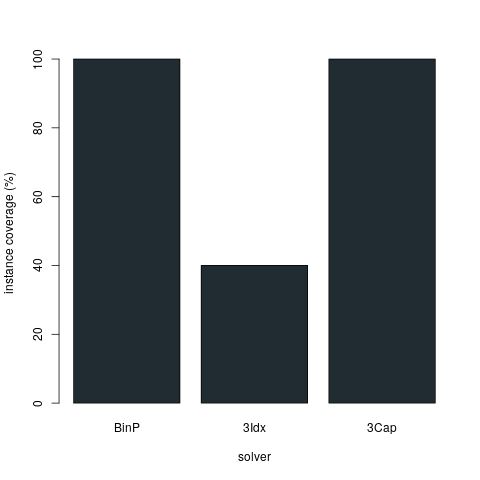
\includegraphics[width=0.3\textwidth]{img/solver_instance_coverage_b=3_m_1200s.png}
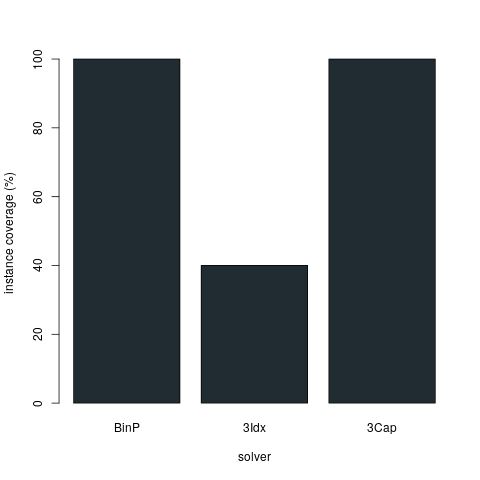
\includegraphics[width=0.3\textwidth]{img/solver_instance_coverage_b=3_m_1800s.png}
\caption*{\textsc{Zeitlimit} $10min$ $\quad\quad\quad$ \textsc{Zeitlimit} $20min$ $\quad\quad\quad$ \textsc{Zeitlimit} $30min$}
% \end{figure}
% \begin{figure}[H]
\begin{subfigure}[b]{0.3\textwidth}
\centering
\resizebox{\textwidth}{!}{
\begin{tabular}{ | l | l | l |}
    \hline
     & \textbf{BinP} & \textbf{3Idx} \\ \hline
    \textbf{Optimal} & $ \textcolor{mygreen}{20 \%}$ & $ \textcolor{red}{10 \%}$ \\ \hline
    \textbf{Laufzeit} & \O $\thinspace \textcolor{red}{583.7 s}$ & \O $\thinspace \textcolor{mygreen}{554.3 s}$ \\ \hline
    \textbf{Abweichung} & \O $\thinspace \textcolor{red}{0.2 \%}$ & \O $\thinspace \textcolor{mygreen}{0.01 \%}$ \\ \hline
\end{tabular}}
\end{subfigure}
% $\quad\quad\quad\quad$
\begin{subfigure}[b]{0.3\textwidth}
\centering
\resizebox{\textwidth}{!}{
\begin{tabular}{ | l | l | l |}
    \hline
     & \textbf{BinP} & \textbf{3Idx} \\ \hline
    \textbf{Optimal} & $ \textcolor{mygreen}{100 \%}$ & $ \textcolor{red}{30 \%}$ \\ \hline
    \textbf{Laufzeit} & \O $\thinspace \textcolor{mygreen}{791.4 s}$ & \O $\thinspace \textcolor{red}{795.4 s}$ \\ \hline
    \textbf{Abweichung} & \O $\thinspace 0.0 \%$ & \O $\thinspace 0.0 \%$ \\ \hline
\end{tabular}}
\end{subfigure}
% \end{figure}
% \begin{figure}[H]
\begin{subfigure}[b]{0.3\textwidth}
\centering
\resizebox{\textwidth}{!}{
\begin{tabular}{ | l | l | l |}
    \hline
     & \textbf{BinP} & \textbf{3Idx} \\ \hline
    \textbf{Optimal} & $ \textcolor{mygreen}{100 \%}$ & $ \textcolor{red}{35 \%}$ \\ \hline
    \textbf{Laufzeit} & \O $\thinspace \textcolor{mygreen}{766.4 s}$ & \O $\thinspace \textcolor{red}{874.0 s}$ \\ \hline
    \textbf{Abweichung} & \O $\thinspace 0.0 \%$ & \O $\thinspace 0.0 \%$ \\ \hline
\end{tabular}}
\end{subfigure}
\end{figure}
\centering
\textbf{3Cap-Heuristik}\linebreak
\centering
Abweichung vom Optimum: \O $\thinspace \boldsymbol{1.02 \%}$\linebreak
\centering
Laufzeit: \O $\thinspace \boldsymbol{0.2 s}$

\pagebreak

\subsection{Vergleich der $b = 3$ Solver (l)}
\label{sec:solver_comp_b=3_l}

\begin{figure}[H]
\centering
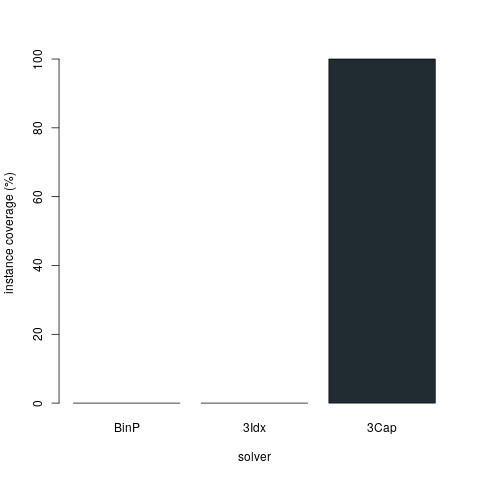
\includegraphics[width=0.3\textwidth]{img/solver_instance_coverage_b=3_l_1800s.png}
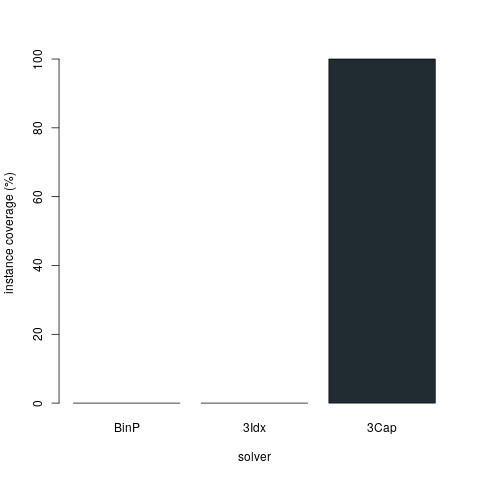
\includegraphics[width=0.3\textwidth]{img/solver_instance_coverage_b=3_l_2700s.png}

\includegraphics[width=0.3\textwidth]{img/na.png}
\caption*{\textsc{Zeitlimit} $30min$ $\quad\quad\quad$ \textsc{Zeitlimit} $45min$ $\quad\quad\quad$ \textsc{Zeitlimit} $60min$}
% \end{figure}
% \begin{figure}[H]
\begin{subfigure}[b]{0.3\textwidth}
\centering
\resizebox{\textwidth}{!}{
\begin{tabular}{ | l | l | l |}
    \hline
     & \textbf{BinP} & \textbf{3Idx} \\ \hline
    \textbf{Optimal} & $ \textcolor{red}{0 \%}$ & $ \textcolor{red}{0 \%}$ \\ \hline
    \textbf{Laufzeit} & $\textcolor{red}{---}$ & $\textcolor{red}{---}$ \\ \hline
    \textbf{Abweichung} & $\textcolor{red}{---}$ & $\textcolor{red}{---}$ \\ \hline
\end{tabular}}
\end{subfigure}
% $\quad\quad\quad\quad$
\begin{subfigure}[b]{0.3\textwidth}
\centering
\resizebox{\textwidth}{!}{
\begin{tabular}{ | l | l | l |}
    \hline
     & \textbf{BinP} & \textbf{3Idx} \\ \hline
    \textbf{Optimal} & $ \textcolor{red}{0 \%}$ & $ \textcolor{red}{0 \%}$ \\ \hline
    \textbf{Laufzeit} & $\textcolor{red}{---}$ & $\textcolor{red}{---}$ \\ \hline
    \textbf{Abweichung} & $\textcolor{red}{---}$ &$\textcolor{red}{---}$ \\ \hline
\end{tabular}}
\end{subfigure}
% \end{figure}
% \begin{figure}[H]
\begin{subfigure}[b]{0.3\textwidth}
\centering
\resizebox{\textwidth}{!}{
\begin{tabular}{ | l | l | l |}
    \hline
     & \textbf{BinP} & \textbf{3Idx} \\ \hline
    \textbf{Optimal} & $-tbd-$ & $-tbd-$ \\ \hline
    \textbf{Laufzeit} & $-tbd-$ & $-tbd-$ \\ \hline
    \textbf{Abweichung} & $-tbd-$ & $-tbd-$ \\ \hline
\end{tabular}}
\end{subfigure}
\end{figure}
\centering
\textbf{3Cap-Heuristik}\linebreak
\centering
Abweichung vom Optimum: $\boldsymbol{tbd}$\linebreak
\centering
Laufzeit: \O $\thinspace \boldsymbol{1.0 s}$
